\documentclass{beamer}
\usetheme{metropolis}

\usepackage[ngerman]{babel}
\usepackage[autostyle=true,german=quotes]{csquotes}
\usepackage[linewidth=1pt]{mdframed}
\usepackage{hyperref}
\usepackage{makecell}
\usepackage{pifont}
\usepackage{tikz}
\usetikzlibrary{positioning, calc, arrows, fit, decorations.pathreplacing, shapes, shapes.multipart, snakes}
\usepackage{verbatim}
\usepackage{textcomp}
\usepackage{centernot}
\usepackage{tabularx}
\usepackage{ulem}
%\usepackage{pdfpages}

\batchmode

\hypersetup{
	colorlinks,
	urlcolor=blue,
	linkcolor=black % for ToC
}
\newenvironment{qaa}[1]{
	#1

	\begin{mdframed}
		\small
}{
	\end{mdframed}
}

\newcommand{\true}{\ding{51}}
\newcommand{\false}{\ding{55}}
\newcommand{\code}[1]{
	\begin{mdframed}
		\verbatiminput{#1}
	\end{mdframed}
}


\title{Tutorium 13: Compiler}
% \subtitle{}
\author{Paul Brinkmeier}
\institute{Tutorium Programmierparadigmen am KIT}
\date{16. Februar 2021}

\begin{document}

\begin{frame}
	\titlepage
\end{frame}

\section{Heutiges Programm}

\begin{frame}{Programm}
	\begin{itemize}
          \item Blatt 11 (Typinferenz und $\textsc{Let}$)
          \item Übersicht Compilerbau
          \item Syntaktische Analyse
	\end{itemize}
\end{frame}

\section{Blatt 11}

\subsection{Aufgabe 2 --- $\lambda$-Terme und ihre allgemeinsten Typen}

\begin{frame}{Aufgabe 2 --- $\lambda$-Terme und ihre allgemeinsten Typen}
  Gegeben seien folgende $\lambda$-Terme:

  \begin{align*}
    t_1 &= \lam{z}{z} \\
    t_2 &= \lam{f}{\lam{x}{\app{f}{x}}} \\
    t_3 &= \lam{f}{\lam{x}{\app{f}{(\app{f}{x})}}} \\
    t_4 &= \lam{x}{\lam{y}{\app{y}{(\app{x}{y})}}}
  \end{align*}

  Führen Sie für jeden dieser Terme eine Typinferenz durch.
\end{frame}

\begin{frame}{Von Typisierungsregeln zu Typinferenz}
  Beim inferieren wird das Pattern-matching der Typen durch die \emph{Unifikation} übernommen.
  Deswegen schreiben wir anstelle von konkreten Typen immer $\alpha_i$ und merken uns die Gleichungen für später:

  \only<1>{
    \begin{equation*}
      \inferrule{
        \Gamma{}, p : \pi \vdash b : \rho
      }{
        \Gamma \vdash \lam{p}{b} : \pi \to \rho
      } \textrm{\textsc{Abs}}
      \;\;
      \leadsto
      \;\;
      {\inferrule{
        \Gamma{}, p : \alpha_j \vdash b : \alpha_k
      }{
        \Gamma \vdash \lam{p}{b} : \alpha_i
      } \textrm{\textsc{Abs}} \atop
      \{ \alpha_i = \alpha_j \to \alpha_k \}}
    \end{equation*}
  }

  \only<2>{
    \begin{equation*}
      \inferrule{
        \Gamma \vdash f : \phi \to \alpha \\
        \Gamma \vdash x : \phi
      }{
        \Gamma \vdash \app{f}{x} : \alpha
      } \textrm{\textsc{App}}
      \;\;
      \leadsto
      \;\;
      {\inferrule{
        \Gamma \vdash f : \alpha_j \\
        \Gamma \vdash x : \alpha_k
      }{
        \Gamma \vdash \app{f}{x} : \alpha_i
      } \textrm{\textsc{App}} \atop
      \{ \alpha_j = \alpha_k \to \alpha_i \}}
    \end{equation*}
  }

  \only<3>{
    \begin{equation*}
      \inferrule{
        \Gamma{}(t) = \tau
      }{
        \Gamma \vdash t : \tau
      } \textrm{\textsc{Var}}
      \;\;
      \leadsto
      \;\;
      {\inferrule{
        \Gamma{}(t) = \alpha_j
      }{
        \Gamma \vdash t : \alpha_i
      } \textrm{\textsc{Var}} \atop
      \{ \alpha_i = \alpha_j \}}
    \end{equation*}
  }
\end{frame}

\begin{frame}{Algorithmus zur Typinferenz}
	\begin{itemize}
		\item Stelle Typherleitungsbaum auf
		\begin{itemize}
			\item In jedem Schritt werden neue Typvariablen $\alpha_i$ angelegt
			\item Statt die Typen direkt im Baum einzutragen, werden Gleichungen in einem Constraint-System eingetragen
		\end{itemize}
		\item Unifiziere Constraint-System zu einem Unifikator
		\begin{itemize}
			\item Robinson-Algorithmus, im Grunde wie bei Prolog
                        \item I.d.R.: Allgemeinster Unifikator (mgu)
		\end{itemize}
	\end{itemize}

	\begin{columns}
		\scriptsize
		\begin{column}{0.3\textwidth}
                  \begin{mathpar}
    \inferrule{
      \Gamma{}(t) = \alpha_j
    }{
      \Gamma \vdash t : \alpha_i
    } \textrm{\textsc{Var}}
                  \end{mathpar}

                  \center
                        Constraint:\\$\{ \alpha_i = \alpha_j \}$
		\end{column}
		\begin{column}{0.3\textwidth}
                  \begin{mathpar}
    \inferrule{
      \Gamma \vdash f : \alpha_j \\
      \Gamma \vdash x : \alpha_k
    }{
      \Gamma \vdash \app{f}{x} : \alpha_i
    } \textrm{\textsc{App}}
                  \end{mathpar}
\center
			Constraint:\\$\{ \alpha_j = \alpha_k \to \alpha_i \}$
		\end{column}
		\begin{column}{0.3\textwidth}
                  \begin{mathpar}
    \inferrule{
      \Gamma{}, p : \alpha_j \vdash b : \alpha_k
    }{
      \Gamma \vdash \lam{p}{b} : \alpha_i
    } \textrm{\textsc{Abs}}
                  \end{mathpar}
                        \center
			Constraint:\\$\{ \alpha_i = \alpha_j \to \alpha_k \}$
		\end{column}
	\end{columns}
\end{frame}

\begin{frame}{Aufgabe 2 --- $t_2$}
  \begin{mathpar}
    \inferrule{
      \only<1>{
        ...
      }
      \only<2->{
        \inferrule{
          \only<2>{
            ...
          }
          \only<3->{
            \inferrule{
              \only<3>{...}
              \only<4->{
                \inferrule{
                  \Gamma(f) = \alpha_2
                }{
                  \Gamma \vdash f : \alpha_6
                } \textsc{Var}
              }
              \\
              \only<4->{
                \inferrule{
                  \Gamma(x) = \alpha_4
                }{
                  \Gamma \vdash x : \alpha_7
                } \textsc{Var}
              }
            }{
              \Gamma \vdash \app{f}{x} : \alpha_5
            } \textsc{App}
          }
        }{
          f : \alpha_2 \vdash \lam{x}{\app{f}{x}} : \alpha_3
        } \textsc{Abs}
      }
    }{
      \vdash \lam{f}{\lam{x}{\app{f}{x}}} : \alpha_1
    } \textsc{Abs}
  \end{mathpar}

  \begin{align*}
    \onslide<3->{\Gamma =& \; f : \alpha_2, x : \alpha_4 } \\
    C =& \; \{ \onslide<5->{ \alpha_1 = \alpha_2 \to \alpha_3,} \onslide<6->{ \alpha_3 = \alpha_4 \to \alpha_5, } \\
    \onslide<7->{  & \;\; \alpha_6 = \alpha_7 \to \alpha_5,} \\
    \onslide<8->{  & \;\; \alpha_6 = \alpha_2, \alpha_7 = \alpha_4} \} \\
  \end{align*}
\end{frame}

\begin{frame}{Aufgabe 2 --- $t_2$}
  \begin{align*}
    C =& \; \{ \alpha_1 = \alpha_2 \to \alpha_3, \alpha_3 = \alpha_4 \to \alpha_5, \\
       & \;\; \alpha_6 = \alpha_7 \to \alpha_5, \\
       & \;\; \alpha_6 = \alpha_2, \alpha_7 = \alpha_4 \} \\
       \\
    \texttt{unify}(C) = \sigma =& [ \su{\alpha_1}{(\alpha_7 \to \alpha_5) \to \alpha_7 \to \alpha_5}, \\
            & \; \su{\alpha_2}{\alpha_7 \to \alpha_5}, \su{\alpha_3}{\alpha_7 \to \alpha_5}, \\
            & \; \su{\alpha_4}{\alpha_7}, \su{\alpha_6}{\alpha_7 \to \alpha_5} ]
  \end{align*}

  Also:

  \begin{equation*}
    \vdash \lam{f}{\lam{x}{\app{f}{x}}} : \sigma(\alpha_1) = (\alpha_7 \to \alpha_5) \to \alpha_7 \to \alpha_5
  \end{equation*}
\end{frame}

\subsection{Aufgabe 3 --- Typabstraktion}

\begin{frame}{Aufgabe 3 --- Typabstraktion}
  In der Typabstraktion $ta(\tau, \Gamma)$ werden nicht \emph{alle} freien Typvariablen von $\tau$ quantifiziert, sondern nur die, die nicht frei in den Typannahmen $\Gamma$ vorkommen.

  Überlegen sie anhand des $\lambda$-Terms $\lam{x}{\lamlet{y}{x}{\app{y}{x}}}$, was passiert, wenn man diese Beschränkung aufhebt!
\end{frame}

\begin{frame}{\textsc{Let}-Polymorphismus: Motivation}
  \begin{equation*}
    \lam{f}{\app{f}{f}}
  \end{equation*}

  \begin{itemize}
    \item Diese Funktion verwendet $f$ auf zwei Arten:
    \begin{itemize}
      \item $\alpha$: Rechte Seite.
      \item $\alpha \to \beta$: Linke Seite, nimmt $f$ als Argument und gibt es zurück.
    \end{itemize}
    \pause
    \item Problem: $\alpha$ und $\alpha \to \beta$ sind nicht unifizierbar!
    \begin{itemize}
      \item \enquote{occurs check}: $\alpha$ darf sich nicht selbst einsetzen.
    \end{itemize}
  \item Idee: Bei jeder Verwendung eines polymorphen Typen erzeugen wir \emph{neue Typvariablen}, um diese Beschränkung zu umgehen.
  \item Anders gesagt: Wir bauen uns ein $f$, was verschiedene Typen annehmen kann.
  \end{itemize}
\end{frame}

\begin{frame}{Typschemata und Instanziierung}
  \only<1>{
    \begin{itemize}
      \item Idee: Bei jeder Verwendung eines polymorphen Typen erzeugen wir \emph{neue Typvariablen}, um diese Beschränkung zu umgehen.
      \item Ein \emph{Typschema} ist ein Typ, in dem manche Typvariablen allquantifiziert sind:
    \end{itemize}

    \begin{align*}
      \phi     & = \forall \alpha_1 . \; ... \; \forall \alpha_n . \tau \\
      \alpha_i & \in FV(\tau)
    \end{align*}

    \begin{itemize}
      \item \emph{Typschemata kommen bei uns immer nur in Kontexten vor!}
      \item Beispiele:
      \begin{itemize}
        \item $\Gamma = f : \forall \alpha . \alpha \to \alpha$
        \item $\Gamma' = g : \forall \alpha . \alpha \to \texttt{int} \to \alpha$
      \end{itemize}
    \end{itemize}

  }

  \only<2>{
    \begin{itemize}
      \item Ein Typschema kann zu verschiedenen Typen \emph{instanziiert} werden.
      \item Allquantifizierte Typvariablen werden mit Typen belegt:
    \end{itemize}

    \begin{align*}
      \forall \alpha . \alpha \to \alpha & \; \succeq \; \text{int} \to \text{int} \;\; (\su{\alpha}{\text{int}}) \\
      \forall \alpha . \alpha \to \alpha & \; \succeq \; \tau \to \tau \;\; (\su{\alpha}{\tau}) \\
      \forall \alpha . \alpha \to \alpha & \; \not\succeq \; \tau \to \sigma \;\; (\tau \neq \sigma) \\
      \forall \alpha . \alpha \to \alpha & \; \not\succeq \; \tau \to (\tau \to \tau) \;\; (\tau \neq \tau \to \tau) \\
      \forall \alpha . \alpha \to \alpha & \; \succeq \; (\tau \to \tau) \to (\tau \to \tau) \;\; (\su{\alpha}{\tau \to \tau})
    \end{align*}
  }
\end{frame}

\begin{frame}{Instanziierung in Haskell}
  Typvariablen in Haskell sind \emph{implizit} allquantifiziert:

  \begin{align*}
    \texttt{(a -> b) -> [a] -> [b]} & \\
    \approx \texttt{forall \{a\} \{b\}. (a -> b) -> [a] -> [b]} &
  \end{align*}

  \only<2>{
    GHCi kann uns diese auch zeigen:

    \code{code/ghci-forall.output}
  }

  \only<3>{
    Wenn wir Parameter in \texttt{map} einsetzen, werden \texttt{a} und \texttt{b} instanziiert:

    \code{code/ghci-map.output}
  }
\end{frame}

\begin{frame}{\textsc{Let}-Polymorphismus}
  \only<1>{
    Um Typschemata bei der Inferenz zu verwenden, müssen wir zunächst die Regel für Variablen anpassen:

    \begin{mathpar}
      \inferrule{
        \Gamma(x) = \phi \\
        \phi \succeq_{\text{frische $\alpha_i$}} \tau
      }{
        \Gamma \vdash x : \alpha_j
      } \textsc{Var} \\
      \text{Constraint:} \; \{ \alpha_j = \tau \}
    \end{mathpar}

    \begin{itemize}
      \item $\succeq_\text{frische $\alpha_i$}$ instanziiert ein Typschema mit $\alpha_i$, die noch nicht im Baum vorkommen.
      \item Jetzt brauchen wir noch eine Möglichkeit, Typschemata zu erzeugen.
    \end{itemize}
  }

  \only<2>{
    Mit einen \textsc{Let}-Term wird ein Typschema eingeführt:

    \begin{mathpar}
      \inferrule{
        \Gamma \vdash t_1 : \alpha_i \\
        \tilde{\Gamma}, x : \tilde{\alpha}_i \vdash t_2 : \alpha_j
      }{ 
        \Gamma \vdash \texttt{let} \;\; x = t_1 \;\; \texttt{in} \;\; t_2 : \alpha_k
      } \textsc{Let}
    \end{mathpar}

    \pause

    \begin{align*}
      \sigma_{let} &= \texttt{unify}(C_{let}) \\
      \tilde{\Gamma} &= \sigma_{let}(\Gamma) \\
      \tilde{\alpha}_i &= ta(\sigma_{let}(\alpha_i), \tilde{\Gamma})
          % C'_{let} &= \{ \alpha_n = \sigma_{let}(\alpha_n) \mid \sigma_{let}(\alpha_n) \;\; \text{ist definiert} \}
    \end{align*}

    $ta(\tau, \Gamma)$ erzeugt ein Typschema, das die Typvariablen aus $\tau$ allquantifiziert, die nicht in $\Gamma$ vorkommen.

    % Constraints: $C'_{let} \cup C_{body} \cup \{ a_j = a_k \}$
  }
\end{frame}

\begin{frame}{Typabstraktion: Beispiel}
  \footnotesize
  \begin{mathpar}
    \inferrule{
      \inferrule{
        \inferrule{
          \inferrule{
            \Gamma'(f) = \alpha_3 \\\\
            \alpha_3 \succeq \alpha_3
          }{\Gamma' \vdash f : \alpha_5} \textsc{\textcolor<4>{red}{Var}} \\
          \inferrule{
            \Gamma'(x) = \text{int} \\\\
            \text{int} \succeq \text{int}
          }{\Gamma' \vdash x : \alpha_6} \textsc{\textcolor<5>{red}{Var}}
        }{
          \Gamma' \vdash \app{f}{x} : \alpha_4
        } \textsc{\textcolor<3>{red}{App}}
      }{
        \Gamma \vdash \lam{f}{\app{f}{x}} : \alpha_2
      } \textsc{\textcolor<2>{red}{Abs}} \\
      \inferrule{
        ...
      }{
        \tilde{\Gamma}, g : \tilde{\alpha}_2 \vdash t : \alpha_7
      }
    }{
      \Gamma \vdash \texttt{let} \;\; g = \lam{f}{\app{f}{x}} \;\; \texttt{in} \;\; t : \alpha_1
    } \textsc{Let}
  \end{mathpar}

  \begin{columns}
    \begin{column}{0.5\textwidth}
      \begin{align*}
        \Gamma  =& \; \textcolor<9>{red}{x : \text{int}} \\
        \Gamma' =& \; x : \text{int}, f : \alpha_3 \\
        C_{let} =& \; \{ \onslide<2->{\alpha_2 = \alpha_3 \to \alpha_4,} \\
                 & \;\;  \onslide<3->{\alpha_5 = \alpha_6 \to \alpha_4,} \\
                 & \;\;  \onslide<4->{\alpha_5 = \alpha_3,} \onslide<5->{\alpha_6 = \text{int}} \}
      \end{align*}
    \end{column}
    \begin{column}{0.5\textwidth}
      \begin{align*}
        \sigma_{let}     =& \; \texttt{unify}(C_{let}) \\
                         =& \; \onslide<6->{\unifier{\su{\alpha_2}{\textcolor<8>{red}{(\text{int} \to \alpha_4) \to \alpha_4}}, ...}} \\
        \tilde{\Gamma}   =& \; \sigma_{let}(\Gamma) = \onslide<7->{\Gamma} = x : \text{int}\\
        \tilde{\alpha}_2 =& \; ta(\sigma_{let}(\alpha_2), \tilde{\Gamma}) \\
                         =& \; ta(\onslide<8->{(\text{int} \to \alpha_4) \to \alpha_4}, \onslide<9->{x : \text{int}}) \\
                         =& \; \onslide<10->{\forall \alpha_4 . (\text{int} \to \alpha_4) \to \alpha_4}
      \end{align*}
    \end{column}
  \end{columns}
\end{frame}

\begin{frame}{Aufgabe 3 --- Typabstraktion}
  \begin{mathpar}
    \inferrule{
      \inferrule{
        \inferrule{
          \Gamma(x) = \alpha_2 \\\\
          \alpha_2 \succeq \alpha_2
        }{
          \Gamma \vdash x : \alpha_4
        } \textsc{\textcolor<1>{red}{Var}} \\
        \inferrule{
          ...
        }{
          \tilde{\Gamma}, y : \tilde{\alpha}_4 \vdash \app{y}{x} : \alpha_5
        } \textsc{App}
      }{
        \Gamma \vdash \lamlet{y}{x}{\app{y}{x}} : \alpha_3
      } \textsc{Let}
    }{
      \vdash \lam{x}{\lamlet{y}{x}{\app{y}{x}}} : \alpha_1
    } \textsc{Abs}
  \end{mathpar}

  \begin{align*}
    \Gamma           =& \; x : \alpha_2 \\
    \sigma_{let}     =& \; \unifier{\su{\alpha_4}{\alpha_2}} \\
    \tilde{\Gamma}   =& \; \sigma_{let}(\Gamma) = \onslide<2->{\Gamma} \\
    \tilde{\alpha}_4 =& \; ta(\sigma_{let}(\alpha_4), \emptyset) = ta(\onslide<3->{\alpha_2}, \emptyset) = \forall \alpha_2 . \alpha_2 \\
                  \neq& \; ta(\alpha_2, x : \alpha_2) = \alpha_2
  \end{align*}
\end{frame}

\begin{frame}{Aufgabe 3 --- Typabstraktion}
  \footnotesize

  \begin{equation*}
    f = \lam{x}{\lamlet{y}{x}{\app{y}{x}}}
  \end{equation*}

  \vfill

  Falsch:

  \begin{columns}
    \begin{column}{0.6\textwidth}
      \begin{mathpar}
        \inferrule{
          \inferrule{
            (...)(y) = \forall \alpha_2 . \alpha_2 \\\\
            \forall \alpha_2 . \alpha_2 \succeq \alpha_8
          }{
            ... \vdash y : \alpha_6
          } \textsc{Var} \\
          \inferrule{
            (...)(x) = \alpha_2 \\\\
            \alpha_2 \succeq \alpha_2
          }{
            ... \vdash x : \alpha_7
          } \textsc{Var}
        }{
          x : \alpha_2, y : \forall \alpha_2 . \alpha_2 \vdash \app{y}{x} : \alpha_5
        } \textsc{App}
      \end{mathpar}
    \end{column}
    \begin{column}{0.4\textwidth}
      Typisierbar, ermöglicht aber kaputten Code, bspw. \\
      $\app{f}{42} \Rightarrow \app{42}{42} \not\Rightarrow$
    \end{column}
  \end{columns}

  \pause
  \vfill

  Richtig:

  \begin{columns}
    \begin{column}{0.6\textwidth}
      \begin{mathpar}
        \inferrule{
          \inferrule{
            (...)(y) = \alpha_2 \\\\
            \alpha_2 \succeq \alpha_2
          }{
            ... \vdash y : \alpha_6
          } \textsc{Var} \\
          \inferrule{
            (...)(x) = \alpha_2 \\\\
            \alpha_2 \succeq \alpha_2
          }{
            ... \vdash x : \alpha_7
          } \textsc{Var}
        }{
          x : \alpha_2, y : \alpha_2 \vdash \app{y}{x} : \alpha_5
        } \textsc{App}
      \end{mathpar}
    \end{column}
    \begin{column}{0.4\textwidth}
      Nicht typisierbar, äquivalent zu $\lam{x}{\app{x}{x}}$
    \end{column}
  \end{columns}
\end{frame}

\subsection{Aufgabe 4 --- Typinferenz, $\textsc{Let}$-Polymorphismus}

\begin{frame}{Aufgabe 4 --- Typinferenz, $\textsc{Let}$-Polymorphismus}
  Bestimmen Sie einen allgemeinsten Typ für den Ausdruck

  \begin{equation*}
    \lamlet{k}{\lam{x}{\lam{y}{x}}}{\appp{k}{a}{(\appp{k}{b}{c})}}
  \end{equation*}

  unter der Typannahme $\Gamma = a : \text{int}, b : \text{bool}, c : \text{char}$.
\end{frame}

\begin{frame}{Aufgabe 4 --- Typinferenz, $\textsc{Let}$-Polymorphismus}
  \begin{mathpar}
    \inferrule{
      \inferrule{...}{
        \Gamma \vdash \lam{x}{\lam{y}{x}} : \alpha_2
      } \textsc{Abs} \\
      \inferrule{...}{
        \Gamma' \vdash \appp{k}{a}{(\appp{k}{b}{c})} : \alpha_7
      } \textsc{App}
    }{
      \Gamma \vdash \lamlet{k}{\lam{x}{\lam{y}{x}}}{\appp{k}{a}{(\appp{k}{b}{c})}} : \alpha_1
    }
  \end{mathpar}

  \only<-6>{
    \begin{align*}
                                      \Gamma =& \; a : \text{int}, b : \text{bool}, c : \text{char} \\
                                     C_{let} =& \; \onslide<2->{\{ \alpha_2 = \alpha_3 \to \alpha_4, ... \}} \\
      \sigma_{let} = \texttt{unify}(C_{let}) =& \; \onslide<3->{\unifier{\su{\alpha_2}{\alpha_6 \to \alpha_5 \to \alpha_6}, ...}} \\
                                    C'_{let} =& \; \onslide<3->{\{ \alpha_2 = \alpha_6 \to \alpha_5 \to \alpha_6, ... \}} \\
                                     \Gamma' =& \; \onslide<4->{\sigma_{let}(\Gamma), k : ta(\sigma_{let}(\alpha_2), \sigma_{let}(\Gamma))} \\
                                \onslide<5->{=& \; \Gamma, k : ta(\alpha_6 \to \alpha_5 \to \alpha_6, \Gamma)} \\
                                \onslide<6->{=& \; \Gamma, k : \forall \alpha_6 . \forall \alpha_5 . \alpha_6 \to \alpha_5 \to \alpha_6}
    \end{align*}
  }

  \only<7->{
    \begin{align*}
      \Gamma  =& \; a : \text{int}, b : \text{bool}, c : \text{char} \\
      \Gamma' =& \; \Gamma, k : \forall \alpha_6 . \forall \alpha_5 . \alpha_6 \to \alpha_5 \to \alpha_6 \\
      \forall \alpha_6 . \forall \alpha_5 . \alpha_6 \to \alpha_5 \to \alpha_6 \succeq & \; \text{bool} \to \text{char} \to \text{bool} \\
      \forall \alpha_6 . \forall \alpha_5 . \alpha_6 \to \alpha_5 \to \alpha_6 \succeq & \; \text{int} \to \text{bool} \to \text{int} \\
      C =& \; \onslide<8->{C'_{let} \cup C_{body} \cup \{ \alpha_1 = \alpha_7 \}}
    \end{align*}
  }
\end{frame}

\section{Einführung in Compilerbau}

% Aufgaben:
% Nicht-SLL(1)-Teilmenge von JSON-Subset ist SLL(n) für n \in 1, 2?
% Rekursiver Abstieg für JSON-Subset
% Rekursiver Abstieg für Klausuraufgabenliste
% Java Bytecode

\begin{frame}{Compiler in ProPa}
	\begin{itemize}
		\item Ein bisschen...
		\begin{itemize}
			\item Lexikalische Analyse (Tokenisierung)
			\item Syntaktische Analyse (Parsen)
			\item \textcolor{gray}{Semantische Analyse (Optimierung)}
			\item Codegenerierung
		\end{itemize}
		\pause
		\item Klausur:
		\begin{itemize}
			\item SLL(k)-Form beweisen
			\item Rekursiven Abstiegsparser schreiben/vervollständigen
			\item First/Follow-Mengen berechnen
			\item Java-Bytecode
				% Zeigen: Java-BC-Aufgabe (16SS), Code-Generierung nächste Mittwoch und Freitag (findet noch statt)
		\end{itemize}
	\end{itemize}
\end{frame}

\subsection{Syntaktische Analyse (18WS)}

\begin{frame}{Syntaktische Analyse (18WS)}
	\begin{align*}
		SGML \to & \;\; \textrm{\texttt{< id >}} \;\; Children \;\; \textrm{\texttt{< / >}}\\
		Children \to & \;\; \epsilon \mid SGML \;\; Children
	\end{align*}

	\begin{equation*}
		\{\textrm{\texttt{<id><id></><id></></>}},\;\;\textrm{\texttt{<id></>}},\;\;...\} \in G
	\end{equation*}

	\pause
	\begin{itemize}
		\item Begründen Sie formal, dass die obige Grammatik nicht in $\textrm{SLL}(1)$-Form ist (3P.).
		\pause
		\item Entwickeln Sie für [eine linksfaktorisierte Version der obigen Grammatik] einen rekursiven Abstiegsparser (16P.).
	\end{itemize}
\end{frame}

\begin{frame}{Java-Bytecode (16SS)}
	\footnotesize
	Übersetzen Sie folgenden Java-Programmausschnitt in Java-Bytecode (10P.):

	\code{code/bytecode16ss.java}

	\pause
	Hinweise:

	\begin{itemize}
		\item Codeerzeugung für bedingte Sprünge: Folien 447ff.
		\item Um eine Bedingung der Form \texttt{!cond} zu übersetzen, reicht es, \texttt{cond} zu übersetzen und die Sprungziele anzupassen.
	\end{itemize}
\end{frame}

% Aufgaben:
% Nicht-SLL(1)-Teilmenge von JSON-Subset ist SLL(n) für n \in 1, 2?
% Rekursiver Abstieg für JSON-Subset
% Rekursiver Abstieg für Klausuraufgabenliste
% Java Bytecode

\section{Compiler}

\subsection{Motivation}

\begin{frame}{Compiler: Motivation}
	\begin{itemize}
		\item Maschine(-nmodell) versteht i.d.R. eingeschränkten Instruktionssatz
		\begin{itemize}
			\item Es gibt/gab zwar auch mal CISC-Maschinen, heute ist sind aber RISC(-ähnliche) Prozessoren am weitesten verbreitet
			\item Gründe: RISC-Prozessoren sind wesentlich einfacher (= billiger) zu bauen
		\end{itemize}
		\item Programme in Maschinensprache sind i.d.R. für Menschen nicht einfach zu Schreiben.
		\pause
		\item Also: Erfinde einfacher zu Schreibende ($\approx$ mächtigere) Sprache, die dann in die Sprache der Maschine übersetzt wird.
		\item Diesen Übersetzungsschritt sollte optimalerweise ein Programm erledigen, da wir sonst auch einfach direkt Maschinensprache-Programme schreiben können.
	\end{itemize}
\end{frame}

\begin{frame}{Compiler}
	\begin{itemize}
		\item Übersetzer für formale Sprachen nennt man \emph{Compiler}
		\item Beispiele:
		\begin{itemize}
			\item C, Haskell, Rust, Go $\to$ X86
			\item Java, Clojure, Kotlin $\to$ Java-Bytecode
			\item TypeScript $\to$ JavaScript
			\item \textcolor{gray}{Python $\to$ Python-AST}
		\end{itemize}
		\pause
		\item \textcolor{gray}{Interpreter kann man auch als Compiler kategorisieren, sie zählen aber i.A. nicht dazu}
		\pause
		\item Single-pass vs. Multi-pass
		\begin{itemize}
			\item Single-pass: Eingabe wird einmal gelesen, Ausgabe währenddessen erzeugt (ältere Compiler)
			\item Multi-pass: Eingabe wird in Zwischenschritten in verschiedene Repräsentationen umgewandelt
			\begin{itemize}
				\item Quellsprache, Tokens, AST, Zwischensprache, Zielsprache
			\end{itemize}
		\end{itemize}
	\end{itemize}
\end{frame}

\subsection{Lexikalische Analyse}

\begin{frame}{Lexikalische Analyse}
	\begin{columns}
		\begin{column}{0.5\textwidth}
			\code{code/lexinput.java}
		\end{column}
		\begin{column}{0.5\textwidth}
			\code{code/lexoutput.java}
		\end{column}
	\end{columns}

	\begin{itemize}
		\item Lexikalische Analyse (Tokenisierung) verarbeitet eine Zeichensequenz in eine Liste von \emph{Tokens}.
		\item Tokens sind Zeichengruppen, denen eine Semantik innewohnt:
		\begin{itemize}
			\item \texttt{int} --- Typ einer Ganzzahl
			\item \texttt{=} --- Zuweisungsoperator
			\item \texttt{x1} --- Variablen- oder Methodenname
			\item \texttt{123} --- Literal einer Ganzzahl
			\item \texttt{"123"} --- String-Literal
			\item etc.
		\end{itemize}
		\item Lösbar mit regulären Ausdrücken, Automaten
	\end{itemize}
\end{frame}

\subsection{Syntaktische Analyse}

\begin{frame}{Syntaktische Analyse}
	\begin{itemize}
		\item Syntaktische Analyse stellt die unterliegende Struktur der bisher linear gelesenen Eingabe fest:
		\begin{itemize}
			\item Blockstruktur von Programmen
			\item Baumstruktur von HTML-Dateien
			\item Header, Inhalt-Struktur von Mails
			\item Verschachtelte mathematische Ausdrücke
		\end{itemize}
		\item Syntaktische Analyse ist das größte Compiler-Thema in PP.
		\pause
		\item Übliche Vorgehensweise (in PP):
		\begin{itemize}
			\item Grammatik $G$ erfinden
			\item ggf. $G$ in einfache Form $G'$ bringen
			\item rekursiven Abstiegsparser für $G'$ implementieren
		\end{itemize}
		\item Alternativ: Parser-Kombinatoren, Yacc, etc.
	\end{itemize}
\end{frame}

\begin{frame}{Beispiel: Mathematische Ausdrücke}
	\begin{columns}
		\begin{column}{0.3\textwidth}
			\begin{equation*}
				1 + 5 * 7 + 6
			\end{equation*}
		\end{column}
		\begin{column}{0.8\textwidth}
                  \Tree [.E [.E 1 ] + [.E [.E [.E 5 ] * [.E 7 ] ] + [.E 6 ] ] ]
		\end{column}
	\end{columns}

	\begin{itemize}
		\item Zu beachten: Punkt-vor-Strich (Präzedenz), Klammerung, etc.
		\item Nicht mehr mit regulären Ausdrücken lösbar
		\item \enquote{Offensichtliche} Grammatik oft nicht einfach zu Parsen
	\end{itemize}
\end{frame}

\begin{frame}{Beispiel: Mathematische Ausdrücke}
	\begin{equation*}
		E \to \;\; \textrm{\texttt{num}} \mid \textrm{\texttt{(}} \;\; E \;\; \textrm{\texttt{)}}
		 \mid E \;\; \textrm{\texttt{+}} \;\; E
		 \mid E \;\; \textrm{\texttt{*}} \;\; E
	\end{equation*}

	\pause

	\begin{columns}
		\begin{column}{0.5\textwidth}
			\begin{figure}
				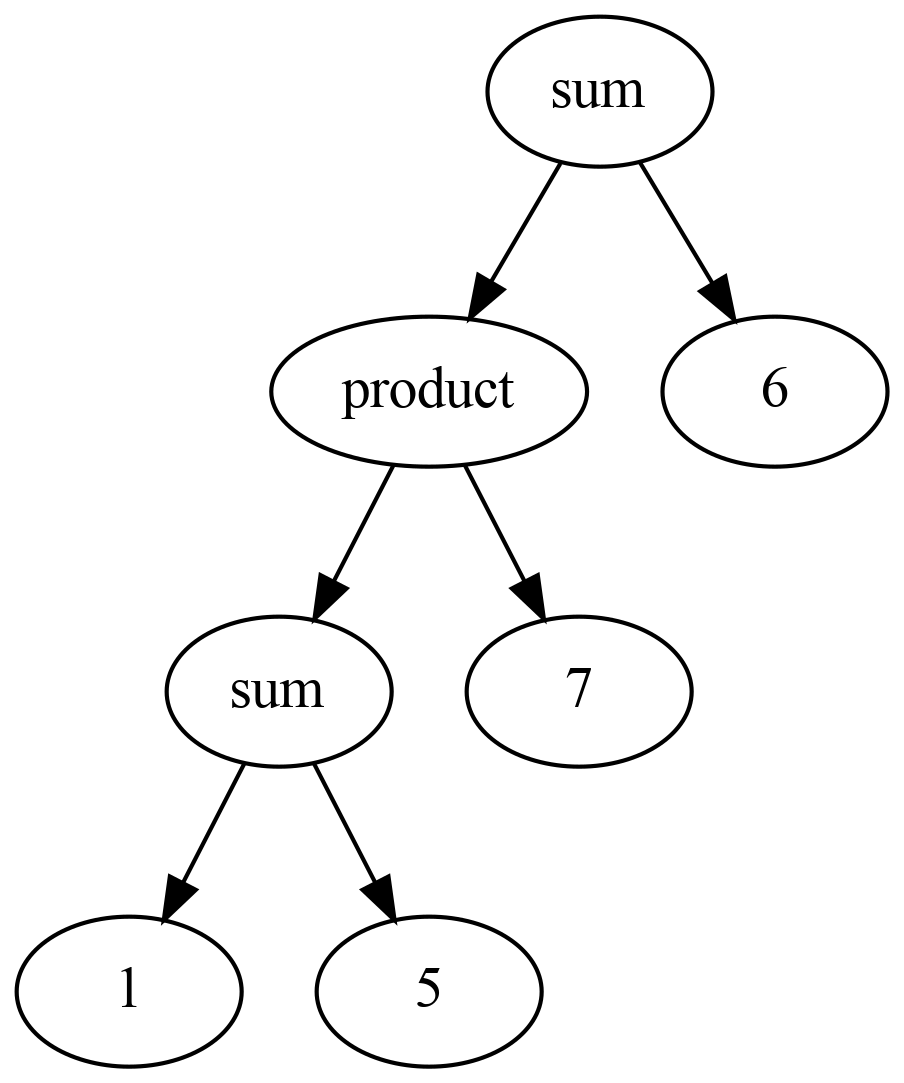
\includegraphics[width=0.65\textwidth]{images/baumstruktur2.png}
			\end{figure}
		\end{column}
		\begin{column}{0.5\textwidth}
			\begin{figure}
				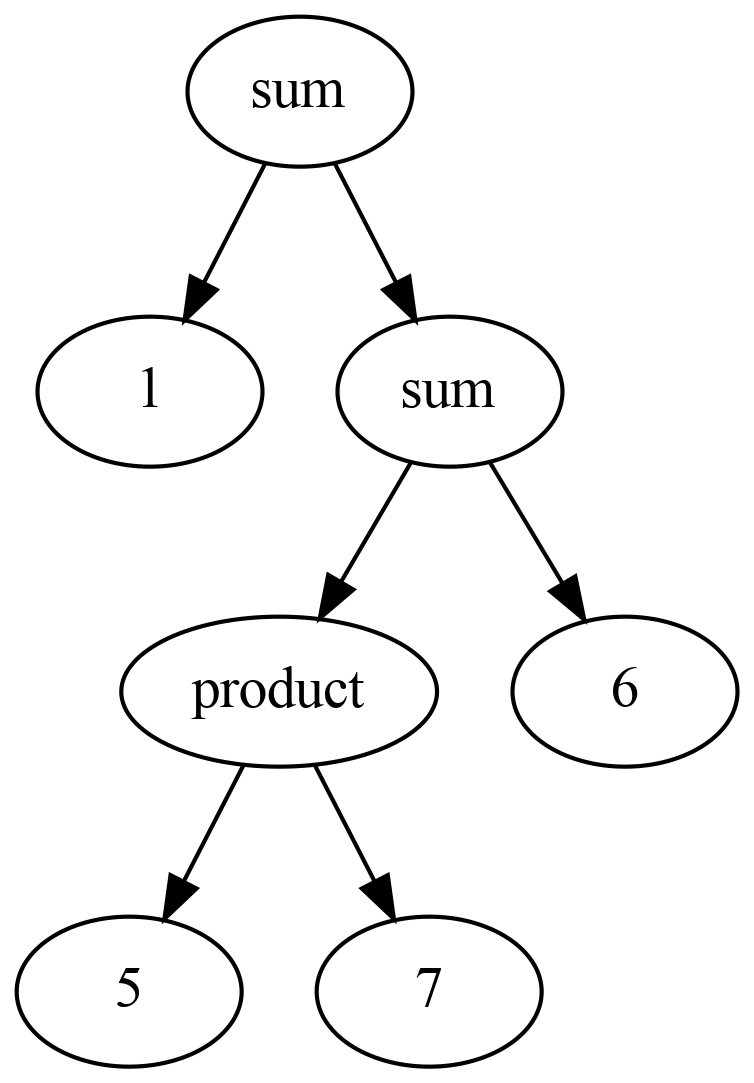
\includegraphics[width=0.65\textwidth]{images/baumstruktur.png}
			\end{figure}
		\end{column}
	\end{columns}

	\pause

	\begin{itemize}
		\item Ableitungsbaum nicht eindeutig $\leadsto$ schlecht
		\item Ableitungsbaum garantiert nicht Punkt-vor-Strich $\leadsto$ schlecht
	\end{itemize}
\end{frame}

\begin{frame}{Präzedenz, Linksfaktorisierung}
	Wie zeichnen sich \enquote{gute} Grammatiken aus?
	\pause

	Operatorpräzedenz schon in Grammatik definiert:
	\begin{align*}
		E \to & \;\; E \;\; \textrm{\texttt{+}} \;\; T \mid E \;\; \textrm{\texttt{-}} \;\; T \mid T\\
		T \to & \;\; T \;\; \textrm{\texttt{*}} \;\; F \mid T \;\; \textrm{\texttt{/}} \;\; F \mid F\\
		F \to & \;\; \textrm{\texttt{num}} \; | \; \textrm{\texttt{(}} \;\; E \;\; \textrm{\texttt{)}}
	\end{align*}

	\pause

	Vermeidung von Linksrekursion (Linksfaktorisierung):
	\begin{align*}
		E     \to & \;\; T \;\; EList\\
		EList \to & \;\; \epsilon \mid \textrm{\texttt{+}} \;\; T \;\; EList \mid \textrm{\texttt{-}} \;\; T \;\; EList\\
		T     \to & \;\; F \;\; TList\\
		TList \to & \;\; \epsilon \mid \textrm{\texttt{*}} \;\; F \;\; TList \mid \textrm{\texttt{/}} \;\; F \;\; TList\\
		F \to & \;\; \textrm{\texttt{num}} \; | \; \textrm{\texttt{(}} \;\; E \;\; \textrm{\texttt{)}}
	\end{align*}
\end{frame}

\begin{frame}{First-/Followmenge, Indizmenge}
	\footnotesize

	\begin{align*}
		EList \to & \;\; \epsilon \mid \textrm{\texttt{+}} \;\; T \;\; EList \mid \textrm{\texttt{-}} \;\; T \;\; EList
	\end{align*}
	
	Wie können wir bspw. bei $EList$ entscheiden, welche Produktion anzuwenden ist?
	\pause
	\begin{itemize}
		\item $\leadsto$ definiere \emph{Indizmenge} $IM_k(A \to \alpha) = \textrm{First}_k(\alpha \textrm{Follow}_k(A))$
		\item Wenn nächste $k$ Token in $IM_k(EList \to \phi)$ $\leadsto$ weiter mit $\phi$
		\pause
		\item $IM_1(EList \to \; \epsilon) = \textrm{First}_1(\epsilon \textrm{Follow}_1(EList)) = \{ \textrm{\texttt{)}}, \textrm{\texttt{\#}} \}$
		\item $IM_1(EList \to \; \textrm{\texttt{+}} \;\; T \;\; EList) = \textrm{First}_1(\textrm{\texttt{+}} \; T \; EList \; \textrm{Follow}_1(EList)) = \{ \textrm{\texttt{+}} \}$
		\item $IM_1(EList \to \; \textrm{\texttt{-}} \;\; T \;\; EList) = \textrm{First}_1(\textrm{\texttt{-}} \; T \; EList \; \textrm{Follow}_1(EList)) = \{ \textrm{\texttt{-}} \}$
		\pause
		\item $\textrm{First}_k(A)$: Menge an möglichen ersten $k$ Token in $A$
		\item $\textrm{Follow}_k(A)$: Menge an möglichen ersten $k$ Token nach $A$
	\end{itemize}
\end{frame}

\begin{frame}{SLL-Kriterium}
	Grammatik ist in $\textrm{SLL}(k)$-Form\\
	$:\Leftrightarrow \forall A \to \alpha, A \to \beta \in P: IM_k(A \to \alpha) \cap IM_k(A \to \beta) = \emptyset$

	\begin{itemize}
		\item $\textrm{SLL}(k)$: Bei jedem Nichtterminal muss die zu wählende Produktion an den nächsten $k$ Token wählbar sein.
		\item Nichtterminale mit nur einer Produktion sind hier irrelevant
		\item Schwierig daran: $\textrm{Follow}$-Mengen berechnen
	\end{itemize}
	\pause
	\begin{align*}
		E \to & \;\; E \;\; \textrm{\texttt{+}} \;\; T \mid E \;\; \textrm{\texttt{-}} \;\; T \mid T\\
		T \to & \;\; T \;\; \textrm{\texttt{*}} \;\; F \mid T \;\; \textrm{\texttt{/}} \;\; F \mid F\\
		F \to & \;\; \textrm{\texttt{num}} \; | \; \textrm{\texttt{(}} \;\; E \;\; \textrm{\texttt{)}}
	\end{align*}
	
	\begin{itemize}
		\item Begründet formal, dass obige Grammatik nicht $\textrm{SLL}(1)$.
		\item Berechnet $\textrm{Follow}_1(N)$ für $N \in \{ E, T, F \}$.
	\end{itemize}
\end{frame}

\begin{frame}{Rekursive Abstiegsparser}
	\footnotesize
	\begin{align*}
		E     \to & \;\; T \;\; EList\\
		EList \to & \;\; \epsilon \mid \textrm{\texttt{+}} \;\; T \;\; EList \mid \textrm{\texttt{-}} \;\; T \;\; EList\\
		T     \to & \;\; F \;\; TList\\
		TList \to & \;\; \epsilon \mid \textrm{\texttt{*}} \;\; F \;\; TList \mid \textrm{\texttt{/}} \;\; F \;\; TList\\
		F \to & \;\; \textrm{\texttt{num}} \; | \; \textrm{\texttt{(}} \;\; E \;\; \textrm{\texttt{)}}
	\end{align*}
	\begin{itemize}
		\item Yay, unsere Grammatik hat jetzt $\textrm{SLL}(1)$-Form!
		\item Aber was bringt das?
		\pause
		\item $G$ ist jetzt einfach ausprogrammierbar:
		\begin{itemize}
			\item 1 Methode per Nichtterminal: \texttt{parseE()}, \texttt{parseEList()}, ...
			\item \texttt{Token[k]}-Instanzattribut für $k$ langen Lookahead
			\item \texttt{expect(TokenType)}-Methode, um Token zu verarbeiten
		\end{itemize}
		\pause
		\item Vervollständigt \texttt{demos/java/exprparser/ExprParser.java}!
	\end{itemize}
\end{frame}

\subsection{Semantische Analyse}

\begin{frame}{Semantische Analyse}
	\begin{itemize}
		\item PP beschäftigt sich (bis auf Typinferenz) nur kurz mit semantischer Analyse
		\item Hier geht es um Optimierungen, Typchecks, etc.
		\item $\leadsto$ weiterführende (Master-)Vorlesungen am IPD
	\end{itemize}
\end{frame}

\section{Ende}

\begin{frame}{Letzte Folie}
  \begin{itemize}
    \item Morgen, Mi, 17.02. um 14:00: Letzte Vorlesung
    \item Mi, 31.03. um 14:00: Fragestunde mit den Übungsleitern
    \begin{itemize}
      \item Per Zoom, über den Vorlesungslink
    \end{itemize}
    \item Tutoriumsfolien, -code, etc.: \href{https://github.com/pbrinkmeier/pp-tut}{github.com/pbrinkmeier/pp-tut}
    \item Fragen auch gerne an \texttt{pp-tut@pbrinkmeier.de} :)
  \end{itemize}

  \vfill

  Danke für's Kommen und eine gute Prüfungsphase!
\end{frame}

\end{document}
